\section{Examples and exercises}

Here, we explore some examples and delve into rigorous exercises to gain more intuition about minima and maxima.


\subsection{Spot whether the function is increasing or decreasing}

Given the functions, can you spot whether it is increasing or decreasing in the given interval? What are the conditions on the interval for which the function shows a particular behavior?

\begin{enumerate}
    \item Prove that function $f(x)=\log _e\left(x^2+1\right)-e^{-x}+1$ is increasing $\forall x \in R$.\\
\begin{outline}
    Sol. $f(x)=\log _e\left(x^2+1\right)-e^{-x}+1$
$$
\therefore \quad f^{\prime}(x)=\frac{2 x}{1+x^2}+e^{-x}=e^{-x}+\frac{2}{x+\frac{1}{x}}
$$

For $x<0, x+\frac{1}{x}<-2$
$$
\begin{gathered}
\therefore \quad-\frac{1}{2}<\frac{1}{x+\frac{1}{x}}<0 \\
\Rightarrow \quad-1<\frac{2}{x+\frac{1}{x}}<0
\end{gathered}
$$

Also, $e^{-x}>1$
$$
\therefore \quad e^{-x}+\frac{2 x}{1+x^2}>0
$$
$\therefore \quad f(x)$ is strictly increasing function $\forall x \in R$
\end{outline}

\item Find the intervals of decrease and increase for the function
$$
f(x)=\cos \left(\frac{\pi}{x}\right) \text {. }
$$\\

\begin{outline}
The function is defined everywhere except 0, where it becomes oscillatory.
    $x \neq 0$.
$$
\therefore \quad f^{\prime}(x)=-\sin \left(\frac{\pi}{x}\right) \pi\left(-\frac{1}{x^2}\right)=\frac{\pi}{x^2} \sin \left(\frac{\pi}{x}\right)
$$

Therefore, $f$ is differentiable for all $x,(x \neq 0)$.
Here, sign of $f^{\prime}(x)$ is same as that of $\sin \left(\frac{\pi}{x}\right)$.
Thus, $f^{\prime}(x)$ is positive if $\sin \left(\frac{\pi}{x}\right)>0$ and $f^{\prime}(x)$ is negative if $\sin \left(\frac{\pi}{x}\right)<0$
or $\sin \left(\frac{\pi}{x}\right)>0$ if $2 k \pi-\frac{\pi}{x}<(2 k+1) \pi, k \in Z$
and $\sin \left(\frac{\pi}{x}\right)<0$, if $(2 k+1) \pi-\frac{\pi}{x}<(2 k+2) \pi, k \in Z$
Hence, the function $f$ is increasing in the interval $\left(\frac{1}{2 k+1}, \frac{1}{2 k}\right)$ and decreasing in the interval $\left(\frac{1}{2 k+2}, \frac{1}{2 k+1}\right)(k$ being a non-negative integer).

\end{outline}

\item Let $g(x)=f(x)+f(1-x)$ and $f^{\prime \prime}(x)>0, \forall x \in(0,1)$. Find the intervals of increase and decrease of $g(x)$. It is given that $f(x)$ and $g(x)$ are differentiable functions.\\\\

\begin{outline}
    Sol. We have, $g(x)=f(x)+f(1-x)$
$$
\therefore \quad g^{\prime}(x)=f^{\prime}(x)-f^{\prime}(1-x)
$$

Given that $f^{\prime \prime}(x)>0, \forall x \in(0,1)$
It means that $f^{\prime}(x)$ is increasing on $(0,1)$.
Now $g(x)$ is increasing,
$$
\begin{array}{ll}
\therefore & f^{\prime}(x)-f^{\prime}(1-x)>0 \\
\Rightarrow & f^{\prime}(x)>f^{\prime}(1-x) \\
\Rightarrow & x>1-x\left(\text { as } f^{\prime}(x)\right. \text { is increasing) } \\
\Rightarrow & \frac{1}{2}<x<1
\end{array}
$$

So, $g(x)$ is increasing in $\left(\frac{1}{2}, 1\right)$
If $g(x)$ is decreasing,
$$
\begin{array}{ll}
\therefore & f^{\prime}(x)-f^{\prime}(1-x)<0 \\
\Rightarrow & f^{\prime}(x)<f^{\prime}(1-x) \\
\Rightarrow & x<1-x\left(\text { as } f^{\prime}(x)\right. \text { is increasing) } \\
\Rightarrow & 0<x<\frac{1}{2}
\end{array}
$$

So, $g(x)$ is decreasing in $\left(0, \frac{1}{2}\right)$

\end{outline}
\end{enumerate}


\subsection{Applicationos of Monotonicity}

Applications of monotonicity can be used in a lot of places, like root estimation, which can, in turn, accelerate the convergence of root-finding algorithms. We can also prove many stubborn-looking inequalities using this method, which has many real-life applications.

\begin{enumerate}
    \item 
Find the number of roots of the function $f(x)=\frac{1}{(x+1)^3}-3 x+\sin x$.\\\\

\begin{outline}
   Sol. $f(x)=\frac{1}{(x+1)^3}-3 x+\sin x, x \neq-1$. $\therefore \quad f^{\prime}(x)=\frac{-3}{(x+1)^4}-3+\cos x=\cos x-3\left(1+\frac{1}{(x+1)^4}\right)$
Now, $\cos x \in[-1,1]$ and $3\left(1+\frac{1}{(x+1)^4}\right)>3$
$\therefore \quad f^{\prime}(x)<0 \forall x \in R$
So, $f(x)$ is a decreasing function.
Also. $f(x)$ is discontinuous at $x=-1$
The graph of the function is shown in the following figure.

\begin{tikzpicture}
\begin{axis}[
  xlabel={$x$},
  ylabel={$f(x)$},
  axis lines=middle,
  xmin=-2, xmax=2,
  ymin=-6, ymax=3,
  xtick={-2,-1,0,1,2},
  ytick={-1,0,1,2,3},
  domain=-2:2,
  samples=100
]

\addplot[blue, thick, domain=-2:2] {1/(x+1)};

\end{axis}
\end{tikzpicture}




$\therefore f(x)=0$ has two roots one in each of the intervals $(-\infty,-1)$ 
\end{outline}


\item Prove that $\log _e(1+x)<x$ for $x>0$.\\\\

\begin{outline}
    Sol. Let $f(x)=\log _e(1+x)-x$
$\therefore \quad f^{\prime}(x)=\frac{1}{1+x}-1=-\frac{x}{1+x}$
For $\quad x>0, f^{\prime}(x)<0$.
So, $f(x)$ is a strictly decreasing function for $x>0$.
$\therefore \quad f(x)<f(0)$ for $x>0$
or $\quad \log _e(1+x)-x<0 \quad($ as $f(0)=0)$
$\therefore \quad \log _e(1+x)<x$ for $x>0$.
\end{outline}

\item 
Show that $1+x \log _e\left(x+\sqrt{x^2+1}\right) \geq \sqrt{1+x^2}$ for all $x \geq 0$.\\\\

\begin{outline}
    Sol. Let $f(x)=1+x \log _e\left(x+\sqrt{x^2+1}\right)-\sqrt{1+x^2}$
$$
\begin{aligned}
\therefore \quad f^{\prime}(x) & =\log _e\left(x+\sqrt{x^2+1}\right)+x \frac{1+\frac{x}{\sqrt{x^2+1}}}{x+\sqrt{x^2+1}}-\frac{x}{\sqrt{1+x^2}} \\
& =\log _e\left(x+\sqrt{x^2+1}\right) \geq 0 \text { for } x \geq 1
\end{aligned}
$$
$\therefore f(x)$ is an increasing function.
So, for $x \geq 0, f(x) \geq f(0)$
$$
\begin{aligned}
& \Rightarrow \quad 1+x \log _e\left(x+\sqrt{x^2+1}\right)-\sqrt{1+x^2} \geq 0 \\
& \Rightarrow \quad 1+x \log _e\left(x+\sqrt{x^2+1}\right) \geq \sqrt{1+x^2}
\end{aligned}
$$
\end{outline}

\end{enumerate}

\subsection{Chasing Extremas by application of First derivatives}

Here, we get exposed to various examples of maxima minima chasing by various methds.

\begin{enumerate}
    \item \begin{outline}
        Find the points of extrema of the function $f(x)=2 \sec x+3 \operatorname{cosec}_x$ in
(i) $(0, \pi / 2)$
(ii) $(\pi, 3 \pi / 2)$
    \end{outline}

Sol.
$$
\begin{aligned}
& f(x)=2 \sec x+3 \operatorname{cosec} x \\
& f^{\prime}(x)=2 \sec x \times \tan x-3 \operatorname{cosec} x \times \cot x
\end{aligned}
$$

Let $f^{\prime}(x)=0$,
$$
\begin{array}{ll}
\therefore \quad & 2 \frac{\sin x}{\cos ^2 x}=3 \frac{\cos x}{\sin ^2 x} \\
\Rightarrow \quad \tan ^3 x=3 / 2 \\
\Rightarrow \quad \tan x=\left(\frac{3}{2}\right)^{1 / 3} \\
\Rightarrow \quad x=n \pi+\tan ^{-1}\left(\frac{3}{2}\right)^{1 / 3}, n \in Z .
\end{array}
$$
(i) if $x \in(0, \pi / 2)$, then $x=\tan ^{-1}\left(\frac{3}{2}\right)^{1 / 3}$
Now $\lim _{x \rightarrow 0^{+}}(2 \sec x+3 \operatorname{cosec} x) \rightarrow \infty$ and
$$
\lim _{x \rightarrow \frac{\pi}{2}^{-}}(2 \sec x+3 \operatorname{cosec} x) \rightarrow \infty
$$
$\therefore \quad x=\tan ^{-1}\left(\frac{3}{2}\right)^{1 / 3}$ is point of minima.
(ii) if $x \in(\pi, 3 \pi / 2)$, then $x=\pi+\tan ^{-1}\left(\frac{3}{2}\right)^{1 / 3}$
Now $\lim _{x \rightarrow \pi^*}(2 \sec x+3 \operatorname{cosec} x) \rightarrow-\infty$
$$
\lim _{x \rightarrow \frac{3 \pi^{-}}{2}}(2 \sec x+3 \operatorname{cosec} x) \rightarrow-\infty
$$
$\therefore \quad x=\pi+\tan ^{-1}\left(\frac{3}{2}\right)^{1 / 3}$ is point of maxima.


\item \textbf{(Non-differentiable functions)} Find the minima of the function $f(x)=\{x\}$


As we can see the graph of this function is: 

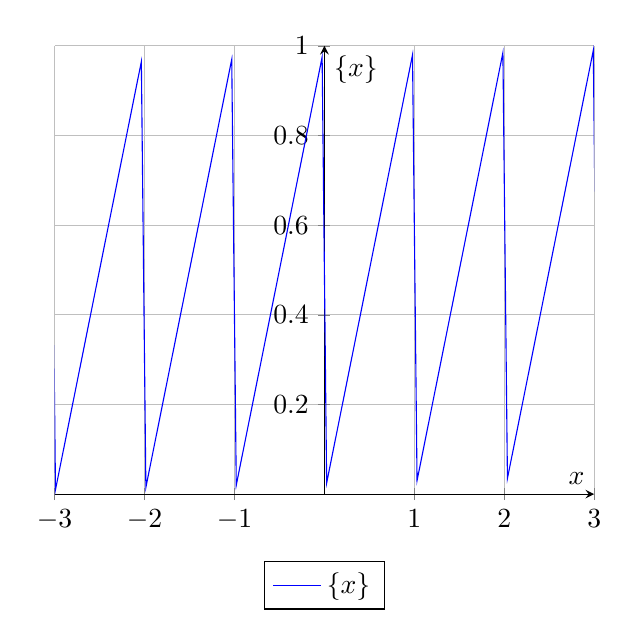
\begin{tikzpicture}
    \begin{axis}[
        xlabel={$x$},
        ylabel={$\{x\}$},
        xmin=-3, xmax=3,
        ymin=0, ymax=1,
        axis lines=middle,
        grid=both,
        legend style={at={(0.5,-0.15)},anchor=north}
    ]
    
    \addplot[blue, domain=-5:5, samples=200] {x - floor(x)};
    \legend{$\{x\}$}
    
    \end{axis}
\end{tikzpicture}

So, we can see that the minima occur at integral points. 
\end{enumerate}